\documentclass[12pt,a4paper]{article}
\usepackage[utf8]{vietnam}
\usepackage{enumerate}
\usepackage[margin=1in]{geometry}
% \usepackage{fixltx2e} %Provide \textsubscript
\usepackage{amsmath, amssymb, amsfonts}
\usepackage{color}
\usepackage{hyperref}
\usepackage{float}
% \usepackage{mathptmx} %Use Times New Roman fonts but not works perfectly
%\usepackage{pgfplots}
\usepackage{indentfirst}
\usepackage{graphicx}

\begin{document}
\begin{center}
	\textbf{Đề tài}
\end{center}

Tham khảo Jame Stewart, Troy Day, Biocalcuclus-Calculus for life sience.
\begin{enumerate} [1.]
	\item Tìm hiểu về \textbf{Cerebral blood flow} trong ví dụ 4, phần 6.1.
	\item Tiềm hiểu về \textbf{Survival an Renewal; Cardiac output; Blood flow} phần 6.3.
\end{enumerate}


\textbf{Yêu cầu:} Hiểu được các thuật ngữ và cách tính. Nêu ví dụ cho mỗi phần, không dùng lại ví dụ của sách.
\newpage
\begin{center}
	\textbf{Lời nói đầu}
\end{center}

Giải tích 1 là một môn đại cương quan trọng đối với các sinh viên ngành Kỹ thuật – Công nghẹ nói chung và sinh viên trường Đại học Bách Khoa nói riêng. Vì thế, việc dành ra một khoảng thời gian lớn để học hỏi lý thuyết và nghiên cứu môn học này là một điều tất yếu, để các sinh viên có một nền móng vũng chắc trong các môn KHTN, tạo tiền đề cho sinh viên học tốt các môn chuyên ngành sau này.\newline


Ở Bài tập lớn này nhóm chúng em đã hiểu được các thuật ngữ và cách tính của:\\
+ Lưu lượng máu não\\
+ Sự tồn tại và thay mới\\
+ Cung lượng tim ( Lượng máu tim bơm ra trong một đơn vị thời gian)\\
+ Lưu lượng máu \\


\textbf{Nhận xét của GVHD:}

\newpage
\begin{center}
	\textbf{Lời cám ơn}
\end{center}

Trong suốt quá trình thực hiện bài tập lớn, nhóm chúng tôi đã nhận được rất nhiều sự quan tâm và ủng hộ, giúp đỡ tận tình của thầy cô, anh chị em và bạn bè.


Ngoài ra, nhóm cũng xin gửi lời tri ân chân thành nhất đến thầy Võ Trần An và cô Trần Thị Ngọc Huyền, là những giảng viên hướng dẫn cho đề tài  này. Nhờ có thầy cô hết lòng chỉ bảo mà nhóm đã hoàn thành bài tập lớn đúng tiến độ và giải quyết tốt những vướng mắc gặp phải. Sự hướng dẫn của thầy cô đã là kim chỉ nam cho mọi hành động của nhóm và phát huy tối đa được mối quan hệ hỗ trợ giữa thầy  và trò trong môi trường giáo dục.


Lời cuối, xin một lần nữa gửi lời cảm ơn sâu sắc đến cá nhân, các thầy cô đã dành thời gian chỉ dẫn cho nhóm. Đây chính là niềm tin và là nguồn động lực to lớn để nhóm có thể đạt được thành quả này.

\newpage
\begin{center}
\tableofcontents
\end{center}

\newpage
\addcontentsline{toc}{section}{CHƯƠNG 1: MỞ ĐẦU}
\section*{CHƯƠNG 1: MỞ ĐẦU}

\newpage
\addcontentsline{toc}{section}{CHƯƠNG 2: CƠ SỞ LÝ THUYẾT}
\section*{CHƯƠNG 2: CƠ SỞ LÝ THUYẾT}
\setcounter{section}{2}
\subsection{Cerebral Blood Flow (Lưu lượng máu não)}
\begin{enumerate}[a/]
	\item \textbf{Định nghĩa}
	      \begin{flushleft}
		      CBF được định nghĩa là thể tích máu chảy trên một đơn vị khối lượng trong
		      một đơn vị thời gian trong mô não và thường được biểu thị bằng đơn vị $ml$\ máu/($100g$\textsubscript{mô}.phút).
		      Ngoài ra, người ta có thể biểu thị CBF dưới dạng lưu lượng trên một đơn vị thể tích mô não,
		      do đó tính bằng $ml$\ máu/($100ml$\textsubscript{mô}.phút).
	      \end{flushleft}
	\item \textbf{Phương pháp đo lường}
	      \begin{flushleft}
		      Phương pháp đo lưu lượng máu não trong đó bệnh nhân được
		      hít một hỗn hợp khí bao gồm chất đánh dấu có chứa $15\%\ N_2O$
		      \begin{itemize}
			      \item[-] 	Gọi $A(t)$ là nồng độ $N_2O$ trong động mạch được đo khi máu đi vào não và $V(t)$ là nồng độ $N_2O$ trong tĩnh mạch trong máu chảy ra từ não trong tĩnh mạch cổ
			      \item[-] 	Biểu đồ thể hiện tương quan giữa $A(t)$ và $V(t)$ như sau:
	 \begin{figure} [ht]
             \centering
             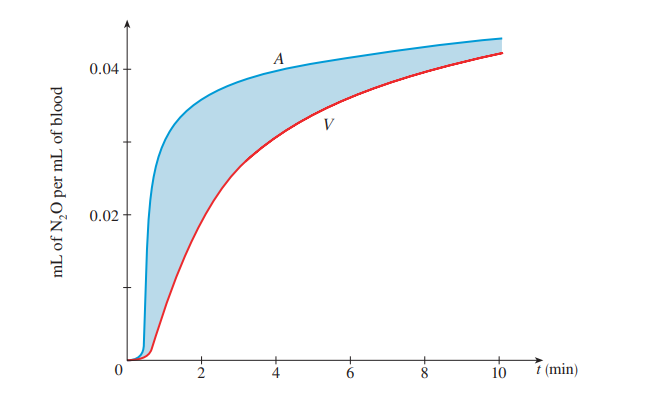
\includegraphics{Images/hình1.png}
             \caption{}
             \label{fig:enter-label}
         \end{figure}
		      \end{itemize}
		      Kí hiệu lưu lượng máu là $F$ (đơn vị $mL$/phút). Xét trong $10$ phút đầu tiên
		      kể từ khi hít, nếu chia khoảng $\left[0,10\right]$ thành các khoảng nhỏ hơn có độ dài bằng nhau $\Delta t$ thì
		      thể tích $N_2O$ chảy qua một điểm trong động mạch trong khoảng thời gian từ $t_{i-1} \to t_i$ xấp xỉ bằng:
	      \end{flushleft}
	      \begin{center}
		      (Nồng độ $N_2O$ trong máu).(Thể tích máu)= $A(t_i)$.($F \Delta t$)
	      \end{center}
	      \begin{flushleft}
		      Dựa theo quy tắc tính tổng Riemann, giả sử như $F$ không đổi thì ta có thể thấy được tổng thể tích khí $N_2O$ đi vào bên trong não bộ trong khoảng 10 phút đầu xấp xỉ là:
		      $$\sum_{i = 1}^{n} A(t_i)F\Delta t = F \sum_{i = 1}^{n} A(t_i) \Delta t$$
		      Khi $n \to \infty$ thì ta sẽ có tổng lượng $N_2O$ được đưa vào não trong $10$ phút đầu tiên là:
		      $$F \int_{0}^{10} A(t)dt$$
		      Bên cạnh đó, tổng lượng $N_2O$ đi ra khỏi não cùng khoảng thời gian là:
		      $$F \int_{0}^{10} V(t)dt$$
		      Theo đó, tổng lượng $N_2O$ thực tế đi vào trong não $10$ phút đầu tiên trong quá trình (Kí hiệu là $Q_B(10)$):
		      $$Q_B(10)=F\int_{0}^{10}\left[A(t)-V(t)\right]dt$$
		      Từ đó ta có:
		      $$F=\frac{Q_B(10)}{\displaystyle \int_{0}^{10}\left[A(t) - V(t)\right]dt}$$
		      Trong đó $\displaystyle \int_{0}^{10}\left[A(t) - V(t)\right]dt$ có thể được tính bằng quy tắc điểm giữa trong tổng Riemann, theo đó:
		      $$\displaystyle \int_{0}^{10}\left[A(t) - V(t)\right]dt = \sum_{i = 1}^{n} \left[A(t_i^*)-V(t_i^*)\right] \Delta t$$
	      \end{flushleft}
	\item \textbf{Ví dụ minh hoạ}
	      \begin{flushleft}
		      Lưu lượng máu trong não bộ của một người được thể hiện bằng lượng khí $N_2O$ được hấp thụ vào não $A(t)$ và lượng $N_2O$ đi ra khỏi não $V(t)$ trong khoảng thời gian 10 phút.
		      Bảng dưới đây cho biết số liệu của lượng khí $N_2O$ trong từng khoảng thời gian:
	      \end{flushleft}
	      \begin{table}[H]
		      \centering
		      \def\arraystretch{1.2}
		      \begin{tabular}{|c|c|c|c|}
			      \hline
			      $t$ & $A(t)$ & $V(t)$ & $A(t) - V(t)$ \\
			      \hline
			      1   & 0.025  & 0.006  & 0.019         \\
			      \hline
			      3   & 0.045  & 0.028  & 0.017         \\
			      \hline
			      5   & 0.048  & 0.039  & 0.009         \\
			      \hline
			      7   & 0.049  & 0.044  & 0.005         \\
			      \hline
			      9   & 0.050  & 0.046  & 0.004         \\
			      \hline
		      \end{tabular}
	      \end{table}
	      \begin{itemize}
		      \item[-] Dùng quy tắc điểm giữa trong tổng Riemann để tính vùng in đậm nằm giữa $A(t)$ và $V(t)$ trong khoảng thời gian đã cho
		      \item[-] Giả sử tổng lượng $N_2O$ hấp thụ bởi não bộ là$ Q_B(10)=60ml$, hãy tính lưu lượng máu não
	      \end{itemize}
	      \centering\underline{Giải}
	      \begin{itemize}
		      \item[-] Bằng quy tắc điểm giữa trong tổng Riemann với $\Delta t=2s$, ta có:
		            $$\int_{0}^{10}\left[A(t)-V(t)\right]dt\approx 2\left[0.019+0.017+0.009+0.005+0.004\right]=0.108$$
	      \end{itemize}
	      \begin{flushleft}
		      Vậy vùng in đậm giữa $A(t)$ và $V(t)$ có giá trị xấp xỉ 0.108 $(mL/mL)$. phút
	      \end{flushleft}
	      \begin{itemize}
		      \item[-] Với $Q_B(10)=60mL$ thì lưu lượng máu não là:
		            $$F=\frac{Q(10)}{\displaystyle \int_{0}^{10}\left[A(t)-V(t)\right]dt} \approx \frac{60}{0.108} \approx 560mL/\text{phút}$$
	      \end{itemize}
\end{enumerate}

\newpage
\subsection{Survival and Renewal (Hàm sống sót và tái sinh)}
\begin{enumerate}[a/]
	\item \textbf{Định nghĩa}
	      \begin{itemize}
		      \item[-] Hàm sống sót (survival function) là một hàm thống kê được sử dụng để miêu tả xác suất một đối tượng nghiên cứu sống sót sau một khoảng thời gian nhất định.
		      \item[-] Hàm tái sinh (renewal function) là một hàm thống kê được sử dụng để mô tả số lần xảy ra của một sự kiện trong một khoảng thời gian nhất định, khi sự kiện được giả định là có tính ngẫu nhiên và không phụ thuộc vào nhau.
	      \end{itemize}
	\item \textbf{Phương pháp tính: (Bài toán dân số)}
	      \begin{flushleft}
		      Giả sử số dân ban đầu là $P_0$, cứ sau $t$ năm sẽ có thêm một tỉ lệ $R(t)$ người dân được thêm vào, tỉ lệ số dân còn lại sau $t$ năm là $S(t)$.
		      Số dân hiện tại (không tính số dân mới thêm vào) còn lại sau $T$ năm:
		      $$S(T).P_0$$
		      Để tính lượng dân số mới thêm vào sau $T$ năm, ta chia khoảng thời gian $\left[0,T\right]$ thành $n$ khoảng bằng nhau có độ dài:
		      $$\Delta t=\frac{T}{n}$$
		      Gọi $t_i$ là điểm cuối bên phải của khoảng thứ $I$, số dân được thêm vào tại thời điểm $t_i$ là:
		      $$R(t_i).\Delta t$$
		      Tỉ lệ những người dân được thêm vào trong khoảng thời gian $t_i$ sống sót sau $T$ năm là:
		      $$S(T-t_i)$$
		      Số dân được thêm vào trong khoảng thời gian $t_i$ sống sót sau $T$ năm là:
		      $$R(t_i).\Delta t.S(T-t_i)$$
		      Theo quy tắc tổng Riemann, số dân được thêm vào sống sót sau $T$ năm là:
		      $$\sum_{i=1}^{n}R(t_i).\ \Delta t.\ S(T-t_i)$$
		      Khi $n \to \infty$, ta có số dân được thêm vào sống sót sau $T$ năm là:
		      $$\int_{0}^{T}S(T-t)\ R(t)dt$$
		      Vậy tổng dân số sau $T$ năm là:
		      $$P(T)=S(T).P_0\ +\ \int_{0}^{T}S(T-t)\ R(t)dt\ (*)$$
	      \end{flushleft}
	      \newpage
	\item \textbf{Ví dụ minh họa}
	      \begin{flushleft}
		      Hiện tại trong một tổ ong nọ có 35000 con ong và sinh sản với tốc độ
		      $R(t)=1500.e^{0.96t}$ con ong/ngày.
		      Nếu tỉ lệ số ong còn lại sau t ngày là $S(t) = e^{-0.5t}$.
		      Hỏi số ong trong tổ sau 1 tuần là khoảng bao nhiêu?
	      \end{flushleft}
	      \begin{center}
            \textbf{\underline{Giải}}
	      \end{center}
	      \begin{flushleft}
		      Ta có: $P_0=35000$, $T=7$(ngày)\\
		      Theo công thức ta tính được số ong trong tổ sau 1 tuần là: %3.06kien
		      $$P(7)=S(7).35000 +\int_0^7S(7-t)R(t)dt$$
		      $$=35000e^{-0.5(7)}+ \int_0^7e^{-0.5(7-t)}1500.e^{0.96t}dt$$
		      $$=3500e^{-3.5}+1500e^{-3.5}\int_0^7e^{0.96t}dt$$
		      $$=3500e^{-3.5}+1500e^{-3.5}(\frac{e^{6.72}}{0.96}-\frac{e^0}{0.96})$$
		      $$\approx40116.16$$\\
		      Vậy ta dự đoán được sẽ có khoảng 40116 con ong trong tổ trong 1 tuần
	      \end{flushleft}
\end{enumerate}

\newpage
\subsection{Blood Flow (Lưu lượng máu chảy)}
\begin{enumerate} [a/]
	\item \textbf{Định nghĩa}
	      \begin{flushleft}
		      Blood Flow (BF) là quá trình chuyển động của dòng máu trong hệ tuần hoàn thông qua sự co bóp cơ tim để di chuyển máu chứa O2 và chất dinh dưỡng đến các mô trong cơ thể và mang máu đã khử O2 và CO2 về lại tim.
	      \end{flushleft}
	\item \textbf{Phương pháp tính }
	      \begin{flushleft}
		      Hình dạng mạch máu được mô tả bằng một ống hình trụ có chiều dài l và bán kính R như hình vẽ:\\
		      % insert hinh ve 2
	        \begin{figure} [ht]
            \centering
            \includegraphics{Images/Hình 2.jpg}
            \caption{}
            \label{fig:enter-label}
        \end{figure}
		      Vận tốc của dòng máu tại vị trí cách trục trung tâm của ống là r: $$V=\frac{P}{4\eta l}(R^2-r^2)$$ \\

		      Trong đó : \begin{enumerate}
			      \item [+]  $\eta $ là độ nhớt của máu
			      \item [+]  P là độ chênh lệch áp suất giữa 2 đầu ống
			            Nếu P và l không đổi thì v là hàm của r có miền [0;R]
		      \end{enumerate}
		      Chia bán kính R thành các bán kính nhỏ hơn có độ dài như nhau là $\Delta R$, diện tích gần đúngcủa vòng có bán kính trong $r_{i-1}$ và bán kính ngoài $r_i$ (như hình vẽ) là: $2\pi r_i \Delta r$ với $\Delta r= r_i-r_{i-1}$\\
		      Với $\Delta r$ rất bé thì vận tốc máu gần như không đổi gần bằng v(r).
		      Thể tích máu chảy qua trong 1 đơn vị thời gian xấp xỉ là:
	\begin{figure}[ht]
            \centering
            \includegraphics[scale=0.5]{Images/Hình-3.1.jpg}
            \caption{}
            \label{fig:enter-label}
        \end{figure}
		      $$(2\pi r, \Delta r)v(r_i)=2\pi r_iv(r_i)\Delta r$$
		      %insert figure 2!!
		      \\
		      Bằng quy tắc tổng Riemann, tổng thể tích máu chảy qua một mặt cắt của một mạch máu trong một đơn vị thời gian là:
		      $$\sum_{i=1}^n2\pi r_iv(r_i)\Delta r$$
		      \\
		      Khi $n \to \infty $ , tổng thể tích máu đi qua mặt cắt của một mạch máu trong một đơn vị thời gian (Kí hiệu: $F$) là:
              \begin{align*}
                F&=\int_0^R 2\pi rv(r)dr\\
                &=\int_0^R 2\pi r\frac{P}{4\eta l}(R^2-r^2)dr\\
                &=\frac{\pi P}{2\eta l}\int_0^R (R^2r -r^3)dr\\
                &=\frac{\pi P}{2\eta l}\left[R^2\frac{r^2}{2}-\frac{r^4}{4}\right]_{r=0}^{r=R}\\
                &=\frac{\pi P}{2\eta l}\left[\frac{R^4}{2}-\frac{R^2}{4}\right]=\frac{\pi PR^4}{8\eta l}
              \end{align*}
		      Biểu thức trên được gọi là định luật Poiseuille’s Law
	      \end{flushleft}
	\item \textbf{Ví dụ minh họa}
	      \begin{flushleft}
		      Sử dụng Định luật Poiseuille’s Law để tính tốc độ dòng chảy trong động mạch nhỏ của con người, trong đó:
		      \\
		      $\eta = 0,027 dyn/cm^2$
		      \\
		      $R= 0,008 cm$
		      \\
		      $l= 2 cm$
		      \\
		      $P= 4000 dyn/cm^2$
	      \end{flushleft}
	      \begin{center}
		      \textbf{\underline{Giải:}}
	      \end{center}
	      \begin{flushleft}
		      Ta có:
		      $$F=\frac{\pi PR^4}{8\eta l}=\frac{\pi 4000.0,008^4}{8.0,027.2}=1,19.10^{-4} cm^3/S=1,19.10^{-4} ml/s$$
		      Áp dụng công thức:
	      \end{flushleft}
	      \begin{center}
		      $v=\frac{F}{A}$ với ( F: lưu lượng máu ; A : Thiết diện mạch)
		      $$=\frac{F}{\pi.R^2}=\frac{1,19.10^{-4}}{\pi . 0,008}=0.59 cm/s$$
	      \end{center}
	      \begin{flushleft}
		      Vậy tốc độ dòng chảy trong động mạch nhỏ của con người là khoảng 0.59 $cm/s$
	      \end{flushleft}
\end{enumerate}

\newpage
\subsection{Cardiac Output (Cung lượng tim)}
\begin{enumerate}[a/]
	\item \textbf{Định nghĩa}
	      \begin{flushleft}
		      Cardiac Output (Cung lượng tim) hay còn được gọi là
		      tần số của dòng máu là lượng máu được tim bơm đi trong một đơn vị thời gian, thường là phút.
	      \end{flushleft}
        %   \vspace{2em}
	\item \textbf{Phương pháp tính}
	      \begin{flushleft}
		      Để tính cung lượng tim, ta sẽ sử dụng phương pháp pha loãng thuốc nhuộm
		      (dye dilution method) bằng cách đưa thuốc nhuộm vào tâm nhĩ phải và được
		      chảy qua tim vào động mạch chủ và quan sát lượng thuốc nhuộm có trong
		      tim trong khoảng thời gian $T$.\\
		      \vspace{1em}
		      Gọi $C(t)$ là nồng độ thuốc nhuộm tại thời điểm $t$, khi chia khoảng thời gian
		      $\left[0,T\right]$ thành các khoảng thời gian nhỏ $\Delta t$ có độ dài bằng
		      nhau thì lượng thuốc nhuộm chảy qua điểm đo trong khoảng thời gian phụ từ $t=t_{i-1}$ đến $t=t_i$, xấp xỉ:\\
		      \begin{center}
			      (Nồng độ thuốc nhuộm trong máu).(thể tích máu)$=c.(t_i).(F\Delta t)$
		      \end{center}
		      Với $F$ là cung lượng tim cần tìm, theo quy tắc tổng Riemann, tổng lượng thuốc nhuộm tại thời điểm $t_i$ là:
		      $$\sum_{i=1}^{n}C(t_i)F\Delta t$$
		      Cho $n \to \infty$, chúng ta có thể thấy lượng thuốc nhuộm là:
		      $$A=\int_{0}^{T}c(t)Fdt=F\int_{0}^{T}c(t)dt$$
		      Do đó cung lượng tim cần tìm là:
		      $$F=\frac{A}{\displaystyle \int_{0}^{T}c(t)dt}$$
	      \end{flushleft}
	\item \textbf{Ví dụ minh họa}
	      \begin{flushleft}
		      Tiêm một lượng thuốc nhuốc nhuộm $8mg$ vào tâm nhĩ phải. Nồng độ thuốc nhuộm ( tính bằng $mg/l$) được đo
		      trong động mạch chủ trong khoảng thời gian 1 giây được thể hiện trong biểu đồ trên.
		      Hãy tính cung lượng tim.
		      \begin{table}[H]
			      \centering
			      \def\arraystretch{1.2}
			      \begin{tabular}{|c|c|c|c|}
				      \hline
				      $t$ & $C(t)$ & $t$ & $C(t)$ \\
				      \hline
				      0   & 0      & 6   & 6.3    \\
				      \hline
				      1   & 0.6    & 7   & 4.8    \\
				      \hline
				      2   & 2.3    & 8   & 2.5    \\
				      \hline
				      3   & 5.9    & 9   & 1.6    \\
				      \hline
				      4   & 9.5    & 10  & 0      \\
				      \hline
				      5   & 8.2    &     &        \\
				      \hline
			      \end{tabular}
		      \end{table}
	      \end{flushleft}
          \newpage
          \begin{center}
            \textbf{\underline{Giải}}
          \end{center}
          \begin{flushleft}
            Qua đề bài ta xác định được $A=8mg$, $T=10$\\
            \vspace{1em}
            Áp dụng quy tắc trung điểm ta có $n=5$ và $\Delta t=2$
            \begin{align*}
                \int_{0}^{10} C(t)dt &\approx \left[C(1)+C(3)+C(5)+C(7)+C(9)\right].\Delta t\\
                &=\left[0.6+5.9+8.2+4.8+1.6\right].2\\
                &=42.2
            \end{align*}
            Ta dùng công thức tính cung lượng tim
            $$F=\frac{A}{\displaystyle \int_{0}^{10} C(t)dt} \approx \frac{8}{42.2} \approx 0.19L/s=11.4L/min$$
          \end{flushleft}
\end{enumerate}

\newpage
\addcontentsline{toc}{section}{CHƯƠNG 3: KẾT LUẬN}
\section*{CHƯƠNG 3: KẾT LUẬN}
\begin{itemize}
	\item[*] \textbf{Ưu điểm:}
	      \begin{itemize}
		      \item[-] Hiểu thêm về ứng dụng của toán học trong những lĩnh vực ngoài đời sống.
		      \item[-] Giúp hiểu thêm về cách sử dụng phần mềm lập trình Latex.
	      \end{itemize}
	\item[*] \textbf{Nhược điểm:}
	      \begin{itemize}
		      \item[-] Thiết kế đoạn code tốn nhiều thời gian, công sức.
	      \end{itemize}
\end{itemize}

\vspace{2em}
Với sự phân công chuẩn bị kỹ lưỡng và cố gắng hết mình, \textbf{nhóm 9} đã hoàn thành đề tài được giao và cho ra kết quả như mong muốn.

\vspace{2em}
\textbf{Qua phần bài tập lớn này nhóm đã:}
\begin{itemize}
	\item[-] Biết được một số thao tác lập trình trên Latex.
	\item[-] Nâng cao sự hứng thú đối với môn học.
	\item[-] Trao dồi kỹ năng học tập và làm việc nhóm.
	\item[-] Nâng cao tinh thần trách nhiệm và thắt chặt tình đoàn kết của các thành viên trong nhóm.
\end{itemize}

\newpage
\addcontentsline{toc}{section}{DANH MỤC TÀI LIỆU THAM KHẢO}
\section*{\small\textbf{DANH MỤC TÀI LIỆU THAM KHẢO}}
\begin{small}
	\begin{enumerate}
		\item J. Stewart and T. Day, Biocalculus: Calculus for Life Sciences. Boston, MA: Cengage Learning, 2015
		\item[] \textcolor{cyan}{\url{https://uotechnology.edu.iq/dep/bme/english/Pages/Lectures/mathmatix/2stage/BIOCALCULUS\%20CALCULUS\%20FOR\%20LIFE\%20SCIENCES\%201ST\%20EDITION\%20C2015.pdf}}
		\item Arthur W. Toga: Brain Mapping - An Encyclopedic Reference, 2015
		\item[] \textcolor{cyan}{\url{https://www.sciencedirect.com/referencework/9780123973160/brain-mapping}}
		\item B. A. Sevast'yanov: Renewal Theory - Journal of Mathematical Sciences, 1975
		\item[] \textcolor{cyan}{\url{https://link.springer.com/article/10.1007/BF01097185}}
		\item David G. Kleinbaum and Mitchel Klein: Survival Analysis: A Self- learning Text, Third Edition
		\item[] \textcolor{cyan}{\url{https://link.springer.com/book/10.1007/978-1-4419-6646-9}}
		\item Jordan King; David R. Lowery: Physiology, Cardiac Output
		\item[] \textcolor{cyan}{\url{https://www.ncbi.nlm.nih.gov/books/NBK470455}}
		\item BS. ĐẶNG HUỲNH ANH THƯ: Sinh lý hệ mạch
		\item[] \textcolor{cyan}{\url{https://admin.ump.edu.vn/uploads/ckeditor/files/CKI\_Timm\%e1\%ba\%a1ch\%20SL\%20h\%e1\%bb\%87\%20m\%e1\%ba\%a1ch.pdf}}

	\end{enumerate}
\end{small}
\end{document}
